%=================
\chapter{Sprint I}
%=================

\section{Sprint planning}
%------------------------
In our first sprint we will implement basic and fundamental parts of the utility. Based on the pre-study, we have decided what preprocessor and parser to use, so the task is to make this work together and achieve the desired functionality.  

\subsection{Duration}
%-----------------
Sprint 1 started September 14th, and lasted until September 27th. To ensure an understanding between our developers and the customer, we will have weekly meetings to show what we have accomplished and discuss further development. 

\subsection{Sprint goal}
%--------------------
The overall goal of the sprint 1 is to create a preliminary design and implement the core of the application. It will be possible to run it and generate the Lua script and therefore it can be used by Wireshark users. The first version will contain only the basic dissector generating features, i.e. parsing simple data structures. Also, some of the preprocessing capabilities will be implemented, such as handling \#include directives. Basic support for configuration will be added.

\subsection{Back log}
%-----------------
The first sprint we will implement eight requirements. Below we have listed each requirement with a time estimate.\\
\autoref{tab:sprint1req} is the sprint backlog for the first phase. \\
\autoref{tab:sprint1time} is the time table for the first phase. \\
\begin{table}[ht] \small \center
\caption{Sprint 1 Requirement FR7-A}
\begin{tabular}{l l c}
	\toprule
	Requirement & Task & Hours \\
	\midrule
	\multirow{4}{5cm}{Command line shall support parameters for c-header file} & Design & 1 \\
	& Implementation & 2 \\
	& Testing & 2 \\
	& Documentation & 4 \\
	\bottomrule
\end{tabular}
\end{table}

\begin{table}[ht] \small \center
\caption{Sprint 1 Requirement FR1-A}
\begin{tabular}{l l c}
	\toprule
	Requirement & Task & Hours \\
	\midrule
	\multirow{4}{5cm}{The utility must support the following basic data types: int, float, char and boolean} & Design & 4 \\
	& Implementation & 8 \\
	& Testing & 8 \\
	& Documentation & 4 \\
	\bottomrule
\end{tabular}
\end{table}

\begin{table}[ht] \small \center
\caption{Sprint 1 Requirement FR2-A}
\begin{tabular}{l l c}
	\toprule
	Requirement & Task & Hours \\
	\midrule
	\multirow{4}{5cm}{The dissector shall be able to display simple structs} & Design & 4 \\
	& Implementation & 8 \\
	& Testing & 8 \\
	& Documentation & 8 \\
	\bottomrule
\end{tabular}
\end{table}

\begin{table}[ht] \small \center
\caption{Sprint 1 Requirement FR3-A}
\begin{tabular}{l l c}
	\toprule
	Requirement & Task & Hours \\
	\midrule
	\multirow{4}{5cm}{The utility shall support \#include} & Design & 2 \\
	& Implementation & 2 \\
	& Testing & 2 \\
	& Documentation & 2 \\
	\bottomrule
\end{tabular}
\end{table}

\begin{table}[ht] \small \center
\caption{Sprint 1 Requirement FR3-B}
\begin{tabular}{l l c}
	\toprule
	Requirement & Task & Hours \\
	\midrule
	\multirow{4}{5cm}{The utility shall support \#define and \#if} & Design & 1 \\
	& Implementation & 2 \\
	& Testing & 6 \\
	& Documentation & 2 \\
	\bottomrule
\end{tabular}
\end{table}

\begin{table}[ht] \small \center
\caption{Sprint 1 Requirement FR7-B}
\begin{tabular}{l l c}
	\toprule
	Requirement & Task & Hours \\
	\midrule
	\multirow{4}{5cm}{Command line shall support for configuration file} & Design & 8 \\
	& Implementation & 8 \\
	& Testing & 8 \\
	& Documentation & 4 \\
	\bottomrule
\end{tabular}
\end{table}

\begin{table}[ht] \small \center
\caption{Sprint 1 Requirement FR4-A}
\begin{tabular}{l l c}
	\toprule
	Requirement & Task & Hours \\
	\midrule
	\multirow{4}{5cm}{Configuration must support valid ranges for struct members} & Design & 6 \\
	& Implementation & 8 \\
	& Testing & 8 \\
	& Documentation & 8 \\
	\bottomrule
\end{tabular}
\end{table}

\begin{table}[ht] \small \center
\caption{Sprint 1 Requirement FR2-D}
\begin{tabular}{l l c}
	\toprule
	Requirement & Task & Hours \\
	\midrule
	\multirow{4}{5cm}{The dissector shall be able to recognize invalid values for a struct member} & Design & 4 \\
	& Implementation & 6 \\
	& Testing & 8 \\
	& Documentation & 4 \\
	\bottomrule
\end{tabular}
\end{table}

\begin{table}[ht] \small \center
\caption{Sprint 1 Requirements \label{tab:sprint1req}}
\begin{tabularx}{\textwidth}{l l X c c}
	\toprule
	& & & \multicolumn{2}{c}{Hours} \\
	\cmidrule(r){4-5}
	\# & Req. & Description & Est. & Act. \\
	\midrule
	1 & FR7-A & Command line shall support parameters for c-header file & 9 & 6\\
	\addlinespace
	2 & FR1-A & Support basic data types: int, float, char, boolean & 24 & 20\\
	\addlinespace
	3 & FR2-A & The dissector shall be able to display simple structs & 28 & 25\\
	\addlinespace
	4 & FR3-A & The utility shall support \#include & 8 & 2\\
	\addlinespace
	5 & FR3-B & The utility shall support \#define and \#if & 11 & 3\\	
	\addlinespace
	6 & FR7-B & Command line shall support for configuration file & 28 & 8\\
	\addlinespace
	7 & FR4-A & Support valid ranges for struct members & 30 & 15 \\
	\addlinespace
	8 & FR2-D & Recognize invalid values for a struct member & 22 & 12\\
	\midrule
	& & Total: & 160 & 91\\
	\bottomrule
\end{tabularx}
\end{table}

\begin{table}[ht] \small \center
\caption{Sprint 1 Timetable\label{tab:sprint1time}}
\begin{tabularx}{\textwidth}{X c c}
	\toprule
	& \multicolumn{2}{c}{Hours} \\
	\cmidrule(r){2-3}
	Description & Est. & Act. \\
	\midrule
	Design & 30 & 10\\
	\addlinespace
	Implementation & 44 & 65 \\
	\addlinespace
	Testing & 50 & 15\\
	\addlinespace
	Documentation & 36 & 1\\
	\midrule
	Total: & 160 & 91\\
	\bottomrule
\end{tabularx}
\end{table} 

\section{Sprint Design}
This section introduces the design of the system modules implemented in sprint 1

\subsection{Utility}
Figure \ref{fig:sp1_class} illustrates the current class diagram for this sprint 1.The CSjark module contains the main method of the utility and is responsible for running the program. The utility will typically start off by using cparser to parse the c-header file given to the utility as a command line argument. Cparser will then use the config module to ensure that the parsing is done correctly after the configuration, and then generate protocols and fields to be used in the CSjark module. The CSjark module then generates a wireshark dissector in LUA code by going through the protocols and fields generated earlier by the cparser module. 

\begin{figure}[here]
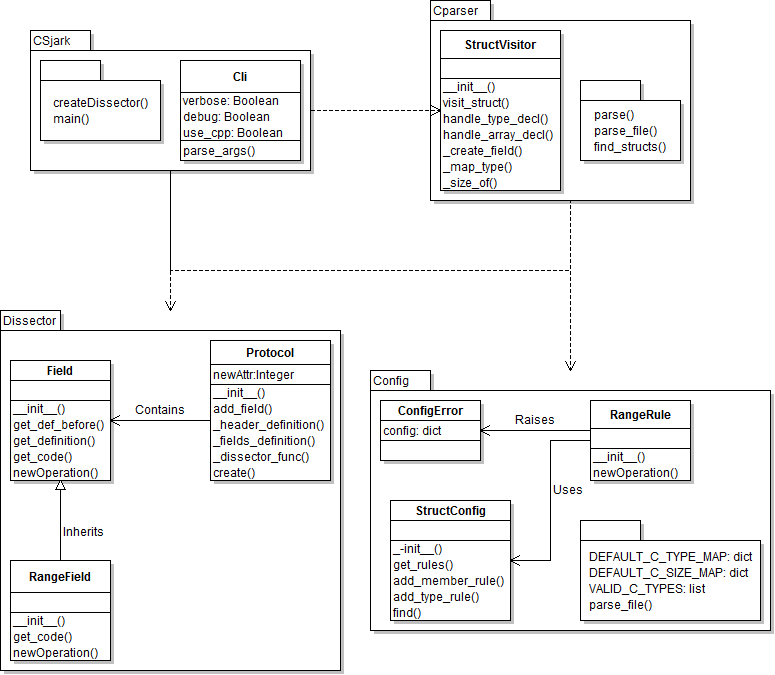
\includegraphics[scale=0.4]{./sprints/img/class_diagram_s1.png}
\caption{Class Diagram}
\label{fig:sp1_class}
\end{figure}

\section{Implementation}

In this sprint we have created a very naive implementation of the utility. It supports the most basic types of C-structs. In addition the utility supports some basic configuration.

We have decided to use YAML as our configuration format. In this sprint we have added support for range specification.
A user can specify the ranges of the members of a struct, from a minimum to a maximum.
In figure \ref{fig:dissector_screenshot} below you can see how Wireshark displays a member that has an invalid range. \newline
\begin{figure}[here]
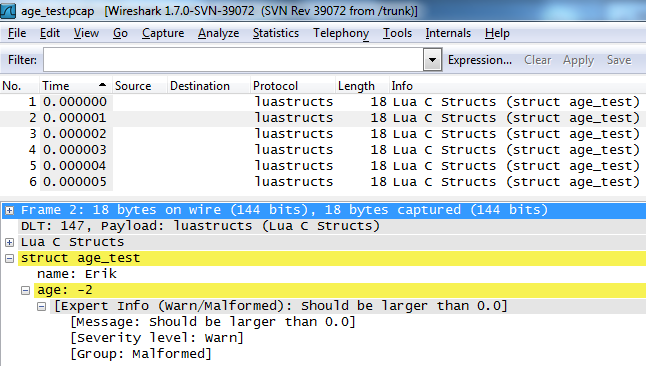
\includegraphics[width=1.2\textwidth]{./sprints/img/wireshark_outofrange.png}
\caption{Wireshark dissector}
\label{fig:dissector_screenshot}
\end{figure}	

The tool uses a command line interface. The user inputs a header-file and optionally a configuration file to the command line, and the program outputs a Lua-script.  Below you can see a figure \ref{fig:cmd_screenshot} that illustrates how the program is run.
\begin{figure}[here]
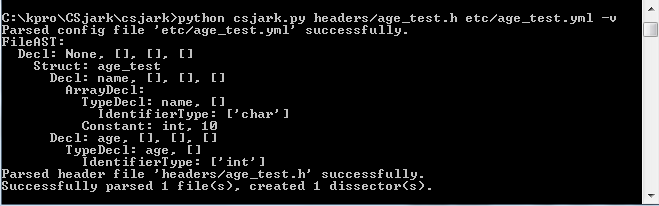
\includegraphics[width=1.2\textwidth]{./sprints/img/cmd_agetest_run.png}
\caption{Command line}
\label{fig:cmd_screenshot}
\end{figure}

\section{Sprint Testing}

\section{Customer Feedback}

\section{Sprint Evaluation}